% Instructions to change to html version:
% Comment out:
%  minipage, multicols,columnbreak, mathbf, hrule
% Replace all: \begin{minipage}% \end{minipage} %\begin{multicols}  %\end{multicols} 
% \columnbreak
 %	%% \begin{framed} %\end{framed} %%\hrule
% Replace \mathbf with	\boldsymbol
% Replace $$ with \[ or \]and $ with \( or \)
% Enclose graphics in figure environments and add captions
% 			search \includegraphics
% Re-tag \df environments as sections, subsections, etc.
% Command Line Code to Create html version:
%First: pdflatex -shell-escape filename.tex                                   
%Second, for each figure: inkscape "filename-figure1.pdf" -o "filename-figure1.png"
% Third: htlatex filename.tex "ht5mjlatex.cfg, charset=utf-8" " -cunihtf -utf8"

\documentclass[10pt]{article}

%\usepackage{tikz, pgf,pgfplots,wasysym,array}
%\usepackage{wasysym,array}

\usepackage{amsmath,amssymb}
\usepackage[hidelinks]{hyperref}

\ifdefined\HCode
  \def\pgfsysdriver{pgfsys-tex4ht-updated.def}
\fi 
%\ifdefined\HCode
%  \def\pgfsysdriver{pgfsys-dvisvgm4ht.def}
%\fi 
\usepackage{tikz}
\usetikzlibrary{calc,decorations.markings,arrows}
\usepackage{pgfplots}

\pgfplotsset{compat=1.12}
\usepackage{myexternalize}
\usetikzlibrary{calc,decorations.markings,arrows}
\usepackage{framed}
\usepackage[none]{hyphenat}

\input{../../../common/1336_header_test.tex}
\begin{document}



\newcommand{\an}{\lbrace a_n \rbrace}
\newcommand{\Sum}{\sum_{n=1}^\infty }
\newcommand{\Sumzero}{\sum_{n=0}^\infty }

\everymath{\displaystyle}

\renewcommand{\myTitle}{	MATH 1336: Calculus III}

\renewcommand{\mySubTitle}{Section 6.3, Part 2: More Practice with Taylor \& Maclaurin Series}
%~\hfill Name: \underline{~~~~~~~~~~~~~~~~~~~~~~~~~~~~~~~~~~~~~~~~~~~~~~~}


%%% Spring 2023: Very short on time, so no error estimation, and remove the trickier two parts of problem 3. Also relabel as Taylor \& Maclaurin Practice Problems, since there probably will not be time for group work.

\lectTitle{\vspace*{-.6in}\myTitle}{\vspace*{.1in}\mySubTitle \vspace*{-.4in}}





%\hspace*{-.8in}%\begin{minipage}{1.25\textwidth}

\setlength{\columnseprule}{.4pt}
\setlength{\columnsep}{3em}

%\begin{framed}
\section*{Taylor/Maclaurin Series Summary:}
\textbf{\underline{\large Key Idea:}}
When \(x\) is close to \(a\) and \(n\) is large: the \(n^{th}\) degree Taylor/Maclaurin polynomial should approximate \(f(x)\) very well!\\

\hrule
\vspace*{.2in}
%\subection*{Taylor/Maclaurin Series Summary:}

%\begin{minipage}{1.125\textwidth}
%\begin{framed}
%\documentclass[11pt]{amsart}
%
%\documentclass[11pt, letterpaper]{article}
%
%\usepackage{amsmath, ulem, graphicx, amsthm, marvosym, multicol}
%\usepackage[left=2cm,right=2cm,top=2cm,bottom=2cm]{geometry}
%
%\renewcommand{\familydefault}{\sfdefault}
%
%%\usepackage{graphics}
%
%%\topmargin -.5in
%%\evensidemargin-.1in
%%\oddsidemargin-.1in
%%\textheight 9in
%%\textwidth 6.5in
%
%\newtheorem*{definition}{Definition}
%%\setlength{\voffset}{-1in}
%
%\everymath={\displaystyle}
%
%%%% 
%% Framed mini-page environment 
%%%%
%\newsavebox{\fmbox}
%   \newenvironment{ans}
%     {\begin{lrbox}{\fmbox}\begin{minipage}{13cm} \textbf{Answer:} \par}
%     {\end{minipage}\end{lrbox}\fbox{\usebox{\fmbox}} \vspace{0.25cm}}
%
%\newcommand{\lcm}{\operatorname{lcm}}
%\newcommand{\ds}{\displaystyle}
%
%\newcommand{\lilspa}{\vspace{.15in}}
%
%\begin{document}

\pagestyle{empty}


%\begin{center}
%{\sc  {\large Taylor Series Summary Sheet}\\
%Math 1336 \& 1337  (Dr. Christine Cole)
%%\\May 16, 2014
%}
%\end{center}
%
%\vspace*{.1in}

{\sc Definition for Taylor Series for \(f(x)\) centered at \(a\):}
\vspace*{-.1in}
\[
\sum_{n=0}^\infty \frac{f^{(n)}(a)}{n!}(x-a)^n  =  f(a) + f^{(1)}(a)(x-a) + \frac{f^{(2)}(a)}{2!}(x-a)^2
\]
\[
   +\ \frac{f^{(3)}(a)}{3!}(x-a)^3+\frac{f^{(4)}(a)}{4!}(x-a)^4+\ldots\\
\]

%\vspace*{.1in}

{\sc Definition for Maclaurin Series for \(f(x)\):}
\vspace*{-.1in}
\[
\sum_{n=0}^\infty \frac{f^{(n)}(0)}{n!}x^n  =  f(0) + f^{(1)}(0)x 
+ \frac{f^{(2)}(0)}{2!}x^2 + \frac{f^{(3)}(0)}{3!}x^3+\frac{f^{(4)}(0)}{4!}x^4+\ldots
\]

\vspace*{-.2in}
%\begin{framed}
{\sc Taylor's Formula / Lagrange's Form of the Remainder:}

\vspace*{-.1in}
\[
R_n(x) = \frac{f^{(n+1)}(z)}{(n+1)!}(x-a)^{n+1}, \qquad \qquad %\textbf{Will NOT be covered in Spring 2023}
\]
\vspace*{-.2in}
%\end{framed}


%\vspace*{.1in}

{\sc Alternating Series Estimation Theorem Formula:}
\vspace*{-.1in}
\[
|R_n| = \left| S - S_n \right | \leq b_{n+1}
\]



\vspace*{.1in}

%
%{\sc Taylor's Formula / Lagrange's Form of the Remainder:}
%
%\vspace*{-.1in}
%\begin{eqnarray*}
%R_n(x) = \frac{f^{(n+1)}(z)}{(n+1)!}(x-a)^{n+1}
%\end{eqnarray*}
%
%
%
%%\vspace*{.1in}
%
%{\sc Alternating Series Estimation Theorem Formula:}
%\vspace*{-.1in}
%\begin{eqnarray*}
%|R_n| = \left| S - S_n \right | \leq b_{n+1}
%\end{eqnarray*}
%
%
%
%\vspace*{.1in}


{\sc Selected Maclaurin Series with Radius of Convergence, \(R\):}

\[
e^x = \sum_{n=0}^\infty \frac{x^n}{n!}  =  1+x+\frac{x^2}{2!}+\frac{x^3}{3!}+\frac{x^4}{4!}+\ldots, \quad R=\infty
\]

\[
\sin(x) = \sum_{n=0}^\infty \frac{(-1)^n x^{2n+1}}{(2n+1)!}  =  x-\frac{x^3}{3!}+\frac{x^5}{5!}-\frac{x^7}{7!}+\frac{x^9}{9!}-\ldots, \quad R=\infty
\]

\[
\cos(x) = \sum_{n=0}^\infty \frac{(-1)^n x^{2n}}{(2n)!}  =  1-\frac{x^2}{2!}+\frac{x^4}{4!}-\frac{x^6}{6!}+\frac{x^8}{8!}-\ldots, \quad R=\infty
\]

\[
\text{Geometric Series: } \frac{1}{1-x} = \sum_{n=0}^\infty x^{n}  =  1+x+x^2+x^3+x^4+\ldots, \quad R=1
\]
\[
\ln(1+x) = \sum_{n=1}^\infty \frac{(-1)^{n-1} x^n}{n}  =  x-\frac{x^2}{2}+\frac{x^3}{3}-\frac{x^4}{4}+\frac{x^5}{5}-\ldots, \quad R=1
\]
%  \\
%\mathrm{Binomial\ Series:\ } (1+x)^k = \sum_{n=0}^\infty\begin{pmatrix} k\\n \end{pmatrix} x^{n}  =  1+kx+\frac{k(k-1)}{2!}x^2+\frac{k(k-1)(k-2)}{3!}x^3+\ldots, \quad R=1\\

%\end{document}



%\end{framed}

\vspace*{-1in}
%\end{minipage}



%\pagebreak
%
%\hspace*{-.5in}
%\begin{minipage}{1.2\textwidth}
%%
%%\setlength{\columnseprule}{.4pt}
%%\setlength{\columnsep}{3em}
%
%\begin{framed}
%%\textbf{New Tests \& Theorems:} 
%%
%%\begin{multicols}{2}
%\includegraphics[height=.89\textheight]{Ch8s7-Taylor-Mac-Summary2}
%\end{framed}
%
%\end{minipage}
%
%

\pagebreak

%\section*{Problems for Group Work}
\section*{Taylor \& Maclaurin Series Practice Problems}

\begin{enumerate}
\item Find a Taylor series for \(f(x) = e^{2x}\) at \(a=3\).\\
Give your answer in the following formats:

%\begin{multicols}{2}
\begin{enumerate}[(a)]

\item The first four non-zero terms of the series, followed by a ``\(+\ldots\)''

\item Using summation notation

\end{enumerate}
%\end{multicols}

\vfill



\item The graphs of \(f\), \(g\), and \(h\) are shown below. Explain why the series shown in Figure \ref{fig:coeffs} cannot be the Maclaurin series for \(f\), \(g\), or \(h\). \label{prob:coeffs}
\[
s(x) = -1+0.3 x - 0.1x^2+0.08x^3+\ldots
\]

\begin{figure}[!h]

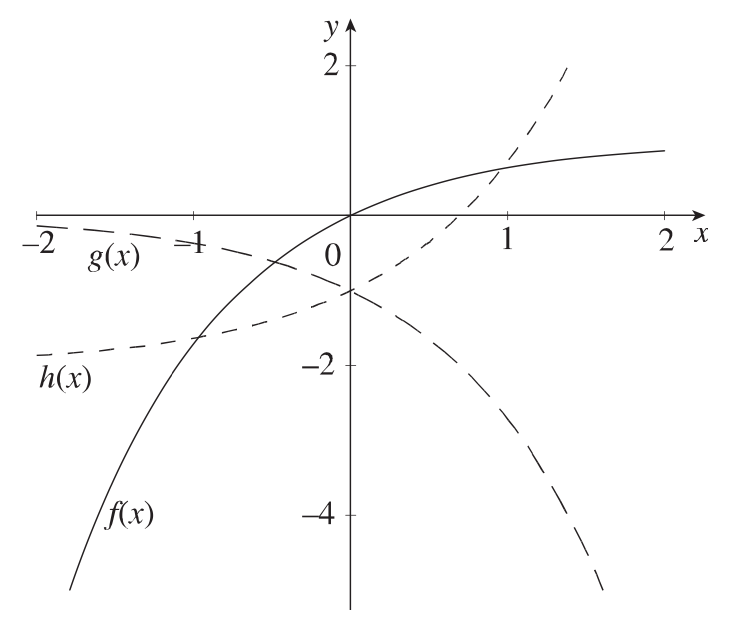
\includegraphics[width=.4\textwidth]{Ch8s7-ws2-prob3.png}
\caption{Graph for use with Problem \ref{prob:coeffs}.}
\label{fig:coeffs}
\end{figure}

\item  Find the series representations for the following functions by any means possible:

%\begin{multicols}{2}
\begin{enumerate}[(a)]

\item \(f(x) = \dfrac{1}{1+x^4}\)

\vspace*{.75in}

\item \(f(x) = \dfrac{1}{1+4x^2}\)

\vspace*{.75in}

\item \(f(x) = \ln\left|\dfrac{1+x}{1-x}\right|\)

\vspace*{.75in}

\item \(f(x) = x^3 \sin x^2\)

\vspace*{.75in}



\end{enumerate}

%\end{multicols}


%\item Let \(f(x) = \Sumzero a_n x^n\) and \(g(x) = \Sumzero b_n x^n\), with \(f(0) = g(0) = 0\).
%\begin{enumerate}[(a)]
%\item What does the condition \(f(0) = g(0) = 0\) mean in terms of the coefficients of the series?
%
%\vfill
%\item Compute \(\lim_{x\rightarrow 0} \frac{f(x)}{g(x)}\)
%\vfill
%
%\item Compute \(\lim_{x\rightarrow 0} \frac{\cos(x^2)-1}{\ln(1+x) - x}\) using the idea from part (b).

%\end{enumerate}

\end{enumerate}
\end{document}
